\section*{Exercise 1 - Inverse transformation and rejection sampling}

\subsection*{Question 1}
Let $Y \sim \text{Exp}(\lambda)$ and $X = Y \mid Y \geq a$ where $a > 0$.

\textbf{CDF of X:}
\begin{align*}
F_X(x) &= P(X \leq x) = P(Y \leq x \mid Y \geq a) = \frac{P(a \leq Y \leq x)}{P(Y \geq a)}
\end{align*}

Since $F_Y(y) = 1 - e^{-\lambda y}$ for $y \geq 0$:
\begin{itemize}
\item For $x < a$: $F_X(x) = 0$
\item For $x \geq a$: 
\begin{align*}
F_X(x) = \frac{F_Y(x) - F_Y(a)}{1 - F_Y(a)} = \frac{(1-e^{-\lambda x}) - (1-e^{-\lambda a})}{e^{-\lambda a}} = 1 - e^{-\lambda(x-a)}
\end{align*}
\end{itemize}

Therefore:
\begin{equation*}
F_X(x) = \begin{cases} 
0 & \text{if } x < a \\ 
1 - e^{-\lambda(x-a)} & \text{if } x \geq a 
\end{cases}
\end{equation*}

\textbf{Quantile function:} Solving $u = F_X(x) = 1 - e^{-\lambda(x-a)}$:
\begin{equation*}
F_X^{-1}(u) = a - \frac{1}{\lambda}\ln(1-u)
\end{equation*}

\textbf{Algorithm:}
\begin{enumerate}
\item Generate $U \sim \mathcal{U}[0,1]$
\item Return $X = a - \frac{1}{\lambda}\ln(1-U)$
\end{enumerate}

\subsection*{Question 2}
We need to show that $X = F_Y^{-1}(F_Y(a)(1-U) + F_Y(b)U)$ has distribution $Y \mid a \leq Y \leq b$.

Let $\alpha = F_Y(a)$ and $\beta = F_Y(b)$. Then:
\begin{equation*}
X = F_Y^{-1}(\alpha + U(\beta - \alpha))
\end{equation*}

Since $U \sim \mathcal{U}[0,1]$, we have $V = \alpha + U(\beta - \alpha) \sim \mathcal{U}[\alpha, \beta]$.

For $a \leq x \leq b$:
\begin{align*}
P(X \leq x) &= P(F_Y^{-1}(V) \leq x) = P(V \leq F_Y(x))\\
&= \frac{F_Y(x) - \alpha}{\beta - \alpha} = \frac{F_Y(x) - F_Y(a)}{F_Y(b) - F_Y(a)}
\end{align*}

This equals $P(Y \leq x \mid a \leq Y \leq b)$ by definition.

\textbf{Detailed explanation of why this equals $P(Y \leq x \mid a \leq Y \leq b)$:}

By the definition of conditional probability:
\begin{align*}
P(Y \leq x \mid a \leq Y \leq b) &= \frac{P(Y \leq x \text{ and } a \leq Y \leq b)}{P(a \leq Y \leq b)}
\end{align*}

Since we're considering $a \leq x \leq b$, the event $\{Y \leq x \text{ and } a \leq Y \leq b\}$ simplifies to $\{a \leq Y \leq x\}$. Therefore:
\begin{align*}
P(Y \leq x \mid a \leq Y \leq b) &= \frac{P(a \leq Y \leq x)}{P(a \leq Y \leq b)}\\
&= \frac{P(Y \leq x) - P(Y < a)}{P(Y \leq b) - P(Y < a)}\\
&= \frac{P(Y \leq x) - P(Y \leq a)}{P(Y \leq b) - P(Y \leq a)} \quad \text{(since $Y$ is continuous)}\\
&= \frac{F_Y(x) - F_Y(a)}{F_Y(b) - F_Y(a)}
\end{align*}

This matches exactly what we obtained for $P(X \leq x)$, confirming that $X$ has the distribution of $Y$ conditioned on $a \leq Y \leq b$.


\textbf{Application to exponential:} Taking $b \to \infty$:
\begin{align*}
X &= F_Y^{-1}((1-e^{-\lambda a})(1-U) + U)\\
&= -\frac{1}{\lambda}\ln(e^{-\lambda a}(1-U))\\
&= a - \frac{1}{\lambda}\ln(1-U)
\end{align*}

For the exponential distribution, we have:
\begin{itemize}
\item $F_Y(y) = 1 - e^{-\lambda y}$ for $y \geq 0$
\item $F_Y(a) = 1 - e^{-\lambda a}$
\item As $b \to \infty$: $F_Y(b) = 1 - e^{-\lambda b} \to 1$
\end{itemize}

Substituting into the formula $X = F_Y^{-1}(F_Y(a)(1-U) + F_Y(b)U)$:
\begin{align*}
X &= F_Y^{-1}((1 - e^{-\lambda a})(1-U) + 1 \cdot U)\\
&= F_Y^{-1}(1 - e^{-\lambda a} - U + Ue^{-\lambda a} + U)\\
&= F_Y^{-1}(1 - e^{-\lambda a} + Ue^{-\lambda a})\\
&= F_Y^{-1}(1 - e^{-\lambda a}(1-U))
\end{align*}

Now, for the exponential distribution, the inverse CDF is:
\begin{equation*}
F_Y^{-1}(p) = -\frac{1}{\lambda}\ln(1-p)
\end{equation*}

Therefore:
\begin{align*}
X &= -\frac{1}{\lambda}\ln(1 - (1 - e^{-\lambda a}(1-U)))\\
&= -\frac{1}{\lambda}\ln(e^{-\lambda a}(1-U))\\
&= -\frac{1}{\lambda}[\ln(e^{-\lambda a}) + \ln(1-U)]\\
&= -\frac{1}{\lambda}[-\lambda a + \ln(1-U)]\\
&= a - \frac{1}{\lambda}\ln(1-U)
\end{align*}

Like in Part 1.

\subsection*{Question 3}
The rejection algorithm simulates from:
\begin{itemize}
\item \textbf{Proposal:} $q(x) = \lambda e^{-\lambda x} \mathbf{1}_{[0,\infty)}(x)$ (standard exponential)
\item \textbf{Target:} $\pi(x) = \lambda e^{-\lambda(x-a)} \mathbf{1}_{[a,\infty)}(x)$ (truncated exponential)
\end{itemize}

The ratio for $x \geq a$:
\begin{equation*}
\frac{\pi(x)}{q(x)} = \frac{\lambda e^{-\lambda(x-a)}}{\lambda e^{-\lambda x}} = e^{\lambda a}
\end{equation*}

Therefore:
\begin{equation*}
M = e^{\lambda a}
\end{equation*}

The acceptance probability is $\frac{1}{M} = e^{-\lambda a} = P(Y > a)$.

\textbf{Expected number of trials:}
\begin{equation*}
E[\text{trials}] = e^{\lambda a}
\end{equation*}

\textbf{Why inversion is preferred for $a \gg 1/\lambda$:}

When $a \gg 1/\lambda$, we have $\lambda a \gg 1$, so $e^{\lambda a} \gg 1$. This means:
\begin{itemize}
\item Rejection algorithm: Expected $e^{\lambda a}$ trials (grows exponentially with $a$)
\item Inversion method: Exactly 1 step regardless of $a$
\end{itemize}

Therefore, inversion is much more efficient for large values of $a$.

\begin{figure}[ht]

\begin{subfigure}{0.45\textwidth}
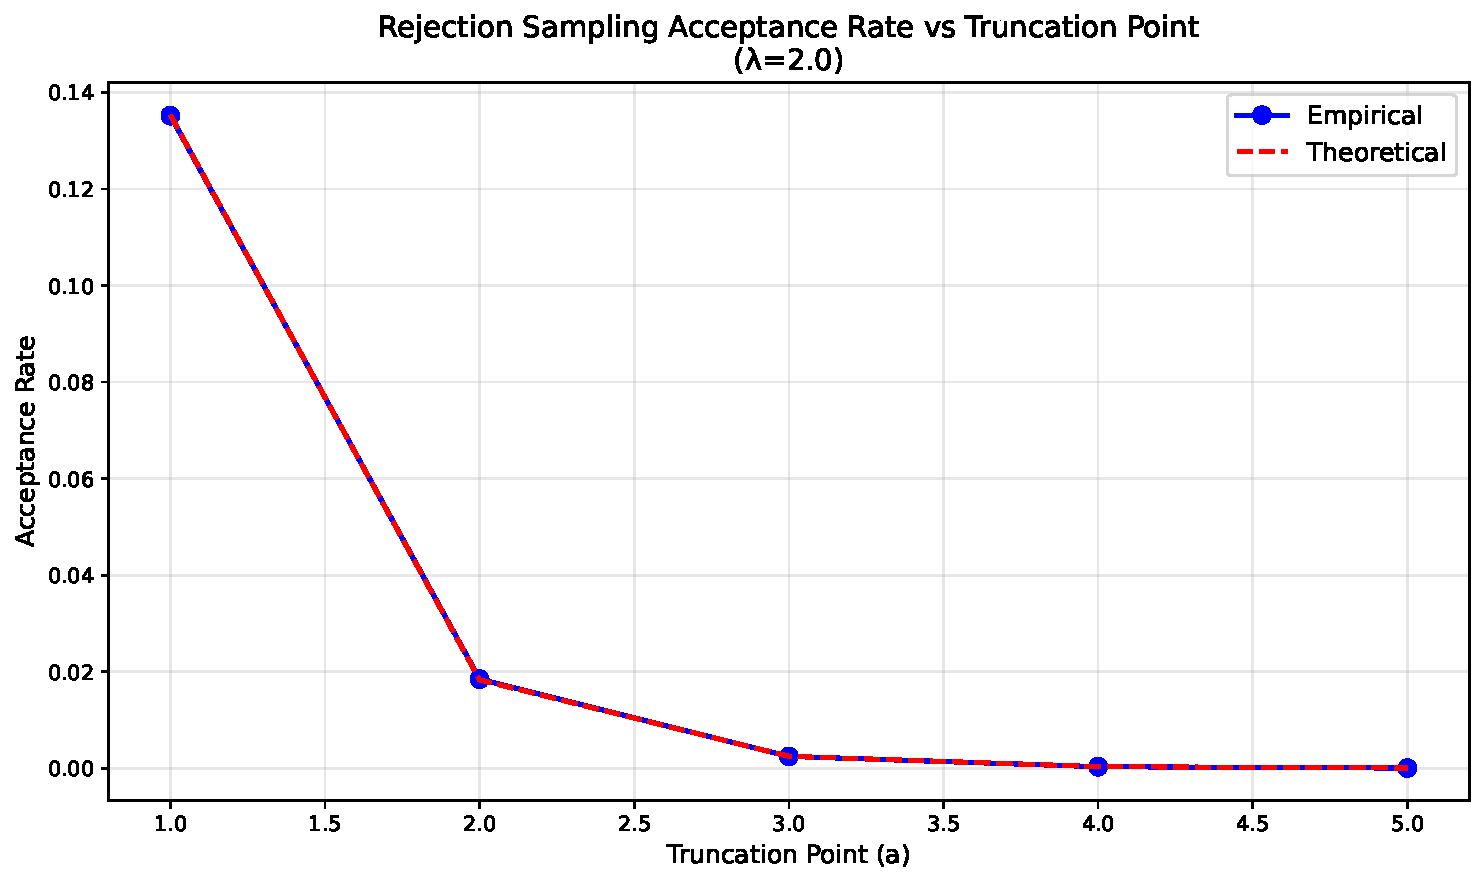
\includegraphics[width=0.9\linewidth, height=6cm]{rejection_sampling_acceptance_rates.pdf} 
\caption{Rejection}
\label{fig:subim1}
\end{subfigure}
\begin{subfigure}{0.45\textwidth}
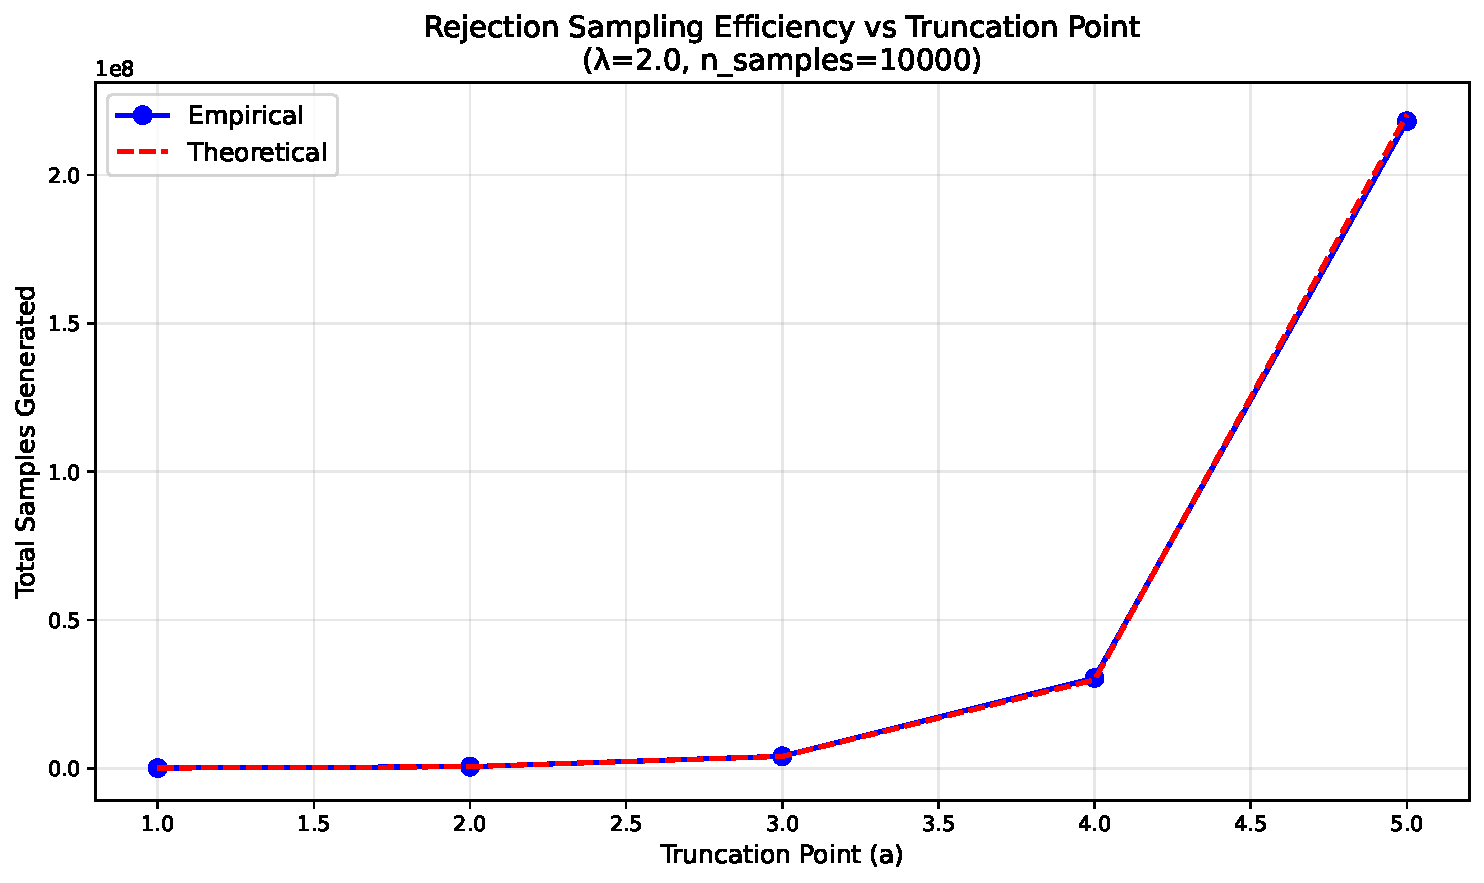
\includegraphics[width=0.9\linewidth, height=6cm]{rejection_sampling_efficiency.pdf}
\caption{Rejection Sampling Efficiency}
\label{fig:subim2}
\end{subfigure}

\caption{Why inversion is preferred for $a \gg 1/\lambda$}
\label{fig:image2}
\end{figure}

\begin{figure}[ht]
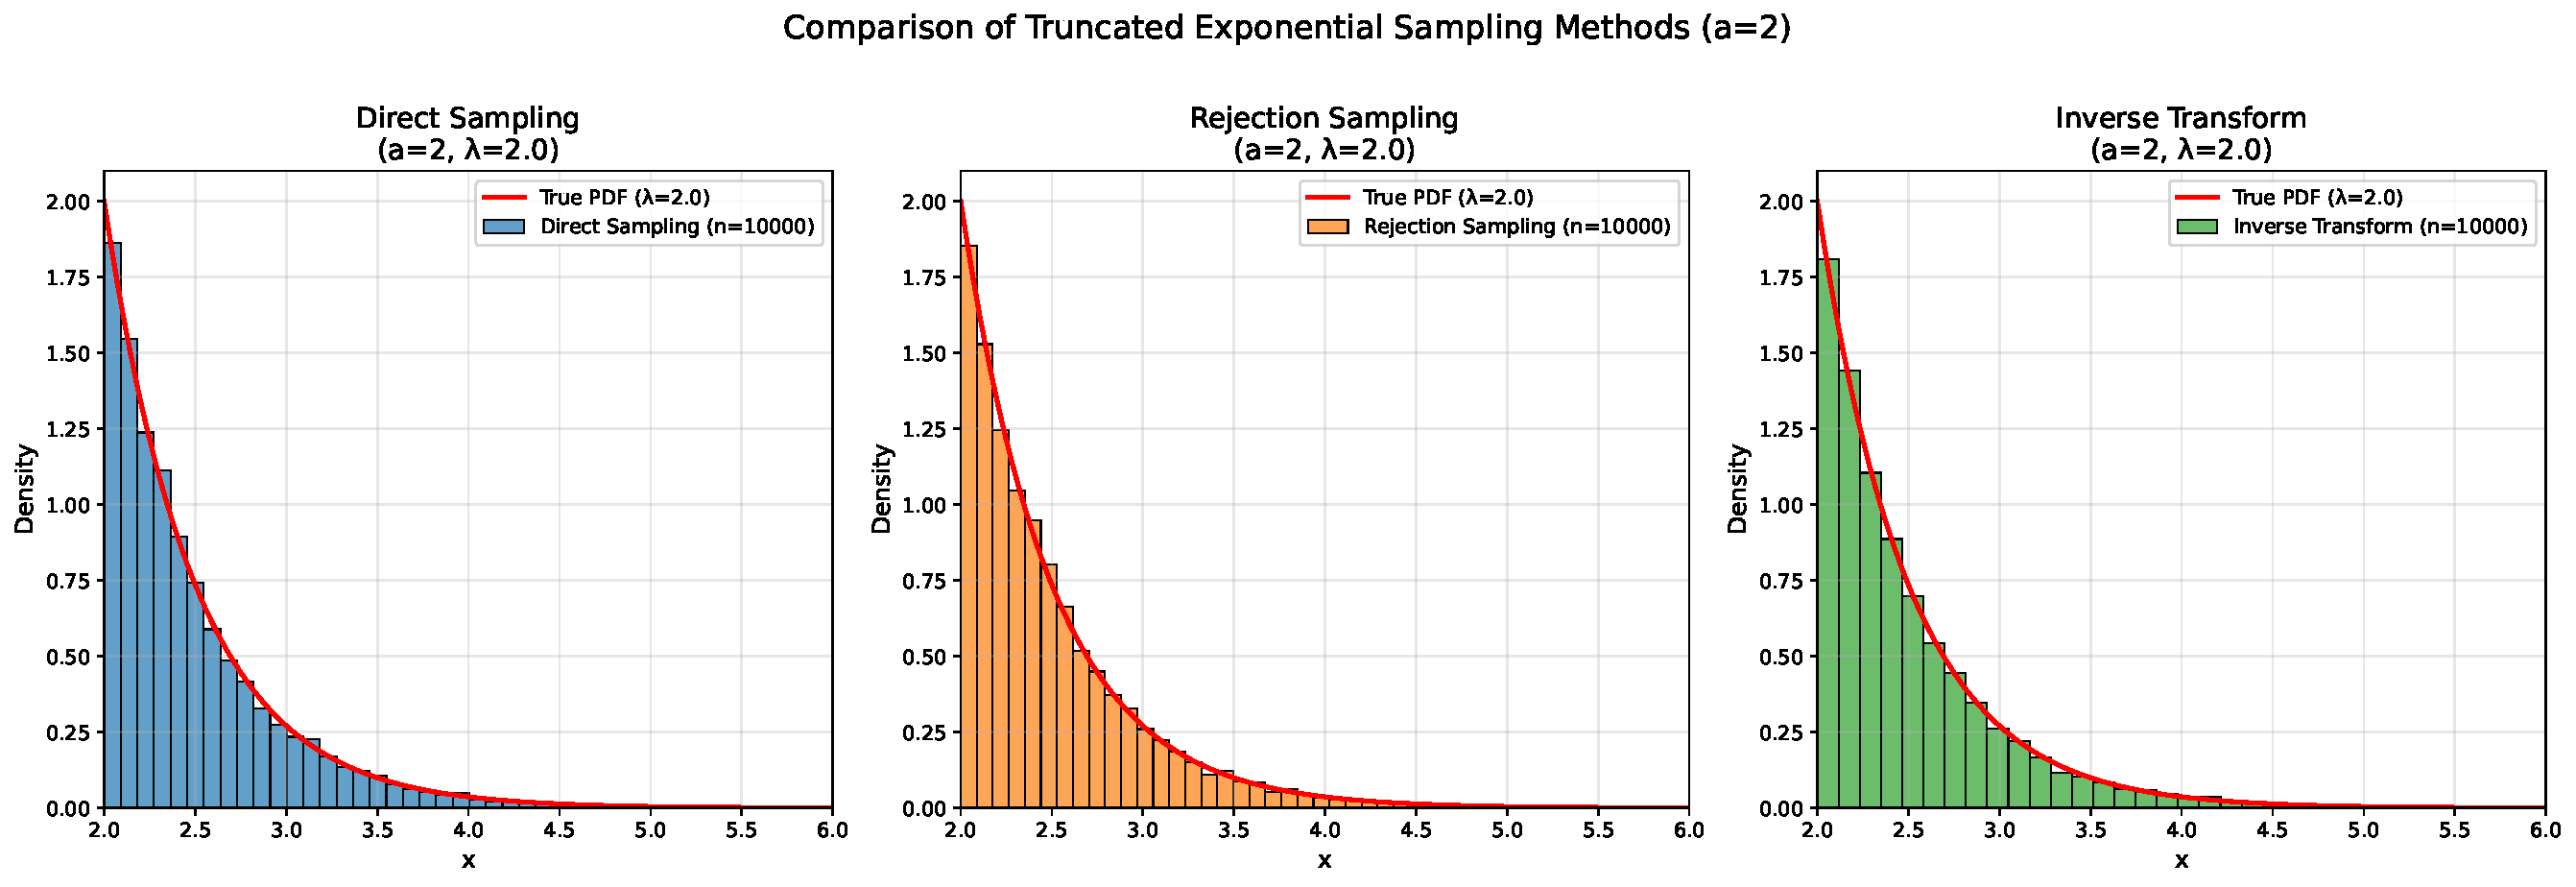
\includegraphics[width=0.9\textwidth]{truncated_exp_comparison_a2.pdf}
\caption{Truncated Exponential Comparison}
\label{fig:figure2}
\end{figure}